% $Id: gui_disres.tex 395 2011-11-17 22:34:59Z cphillip $
%
% Written by Jonas Richiardi, updated by J. Schrouff for v2.0
%_______________________________________________


\chapter{Display Model Performance}
\label{chap:DisRes}
\minitoc

\section{Introduction}

Once a machine (e.g. a classifier or a regression function) has been specified, 
its parameters have been estimated over training data, and its performance has been
evaluated over a testing set using cross-validation, it is necessary to examine the outcome
of the whole procedure in detail. The results windows enables the user to see the model's performance evaluated by different metrics.

Examining model output and parameters is helpful in diagnosing the potentially
bad performance of a particular model. For example, if the machine cannot perform above
chance, it could be due to an inappropriate experimental paradigm, noisy data, insufficient
amount of data, wrong choice of features,  or the wrong choice of machine. It is important to
recognise that any of these factors could cause the modelling to fail. 

Model performance can be reviewed using the `Display Results' GUI. Alternatively, all computed statistics are saved within the PRT structure, in the \texttt{PRT.model(m).output.stats} field, with \texttt{m}, being the index of the model to review.

\section{Launching results display}

Make sure all previous steps have been performed (Data and Design, Chapter~\ref{chap:DataDesign};
Prepare feature set, Chapter~\ref{chap:PrepFeat}; Specify Model and Run Model, Chapter~\ref{chap:ModelCrossV} ).

In the {\tt Review Options} panel of the main PRoNTo window, press {\tt Display Results}. At the `Select PRT.mat' window, navigate to where your {\tt PRT.mat} file is stored (using the left column), and select it. The main results window will open and look as represented in Figure \ref{fig_prt_ui_results_emptyWin}. In the {\tt Model} panel in the top-right corner, the list of models that have been successfully estimated will appear. Note: there will be a `beep' if one or more models were specified but not estimated (`Run model') and their name will appear in the command window.

\begin{figure}[h!]
\begin{center}
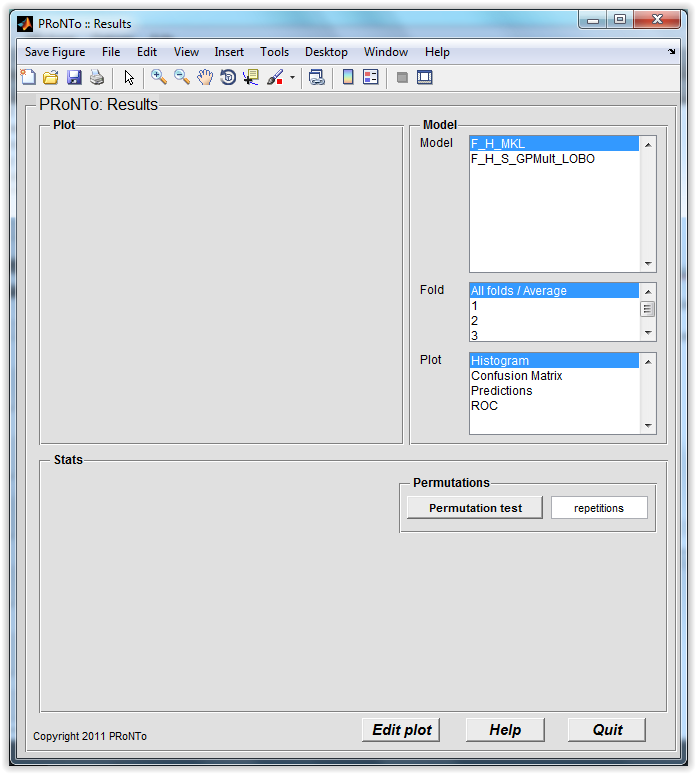
\includegraphics[width=10cm]{images/prt_ui_results_emptyWin.png}
\caption{Initial state of the results display main window.}
\label{fig_prt_ui_results_emptyWin} 
\end{center}
\end{figure}

\section{The main results display window}

The window is divided into three panels; going clockwise from top left to bottom left, they
are:
\begin{description}
\item[Plot]: This panel displays the plots for the various analyses that can be performed on
test results. With the exception of the confusion matrix plot, these cannot be interacted with.
\item[Model]: This panel allows the user to select the model to visualize, whether to visualize a
particular fold or all folds at once, and which plot to produce.
\item[Stats]: The {\tt stats} panel allows the user to visualize a variety of performance metrics (based on the selected fold), including accuracy statistics for classifiers and MSE for regression models. In addition, p-values for these metrics based on permutation tests can also be visualized.
\end{description}

To populate the `Plot' panel, first click on a model in the {\tt Model} selector, then on
`all folds' (or a particular fold) in the {\tt Fold} selector, and finally on a plot
in the {\tt Plot} selector. The next section details the plots available.

The window also comprises `Edit plot', `Help' and `Quit' buttons. The `Edit plot' button exports the displayed plot in an extra window, such
that it can be edited and easily saved. The `Help' button provides information on each panel of the window (not as detailed as in this
manual) and the `Quit' button closes the results window. In addition, the GUI menu comports a `Save figure' option (on the top left) that
acts as a `printscreen' of this window (with white background), which can be saved for records/publications.

\section{Analysing a machine's performance graphically}

Looking at a machine output's graphically can often yield insights into the performance
of the machine. In PRoNTo, plots are different for classification and regression.

\subsection{Classification}

\subsubsection{Predictions plot}

A prediction plot displays, for a particular fold (y-axis), the output value of the machine's
decision function for each test sample (x-axis, e.g., for a linear SVM, this could be $\mathbf{w}^T\mathbf{x}_i + b$,
for a probabilistic classifier this could be a posterior probability $P(\Omega=\omega | \mathbf{x}_i)$). The decision threshold is displayed by a vertical line at the centre of the plot.
A well-performing classifier will yield very different function values for samples of different
classes, i.e. samples from different classes will fall on different sides of the decision threshold. 
%By observing which fold have more or less overlapping function values, it is possible
%to understand which block / subject / condition might have a test distribution of features that
%departs from the training set. 
The inspection, in each fold, of the overlap of function values between classes, can help to identify which of the test blocks/subjects/conditions is atypical with respect to the training set.  
This plot is available for binary classification.


On the plot, each class is represented by a different marker and color, and indicated in the legend.
Figure \ref{fig_prt_ui_results_plots_pred} shows an example predictions plot. 

\begin{figure}[h!]
\begin{center}
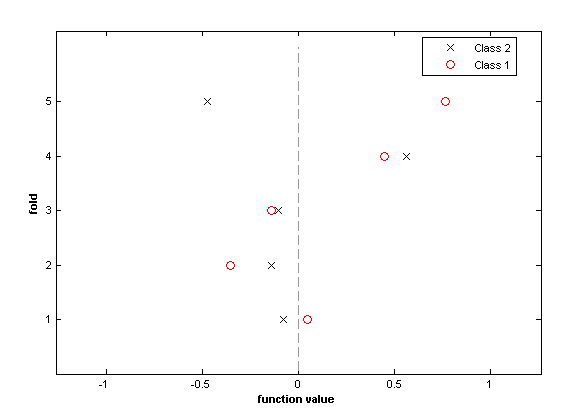
\includegraphics[height=6cm]{images/prt_ui_results_plots_pred.png}
\caption{Example predictions plot for a two-class problem modelled by an SVM.}
\label{fig_prt_ui_results_plots_pred}
\end{center}
\end{figure}

\subsubsection{Receiver Operating Characteristic (ROC) plot}

In two-class classification, there is always a trade-off between class 1
and class 2 errors. Indeed, a classifier predicting class 1 regardless of input
would have excellent accuracy on class 1, but bad accuracy on class2. This is also
known as the sensitivity / specificity trade-off. The 
ROC curve is a graphical depiction of this trade-off, showing how one error rate
varies as a function of the other. An ideal classifier would have an ROC passing
through the top-left corner. The area under curve (AUC) is a summary measure of 
classifier performance, where higher is better (1 represents perfect performance,
0.5 represents random performance). As with all summary measures,
the AUC is but one way of comparing performance of machines, and cannot be used alone
to declare a machine statistically significantly superior to another on a given dataset.

Figure \ref{fig_prt_ui_results_plots_ROC} shows an example of such a plot (Haxby dataset, Faces versus Houses, 4-folds nested CV, LOBO outer CV).

\begin{figure}[h!]
\begin{center}
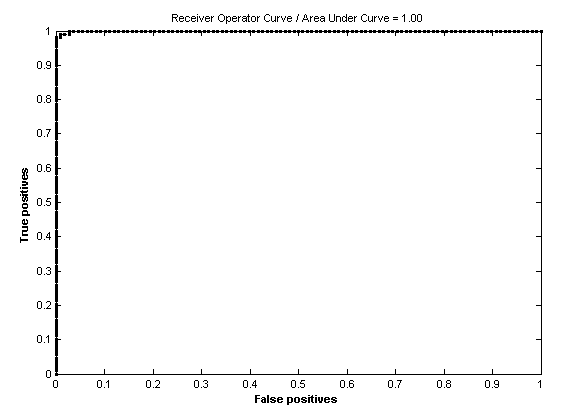
\includegraphics[height=6cm]{images/prt_ui_results_plots_ROC.png}
\caption{Example ROC curve for a two-class problem modelled by an MKL on ROIs.}
\label{fig_prt_ui_results_plots_ROC}
\end{center}
\end{figure}

\subsubsection{Histogram plot}

The histogram plot is a smoothed density version of the predictions
plot, showing how function values are distributed. A good classifier
would have minimal overlap between the densities. The error rate of the
classifier is proportional to the area of the overlap. The ROC curve can 
be thought of as the result of sweeping a decision threshold over the range
of functional values, and recording the joint sensitivity/specificity values
for each decision threshold setting. A typical linear SVM would have a decision
threshold at 0.

Figure \ref{fig_prt_ui_results_plots_hist} shows an example of such a plot for a binary classification (SPM EEG dataset, Faces versus Scrambled, LOBO CV).


\begin{figure}[h!]
\begin{center}
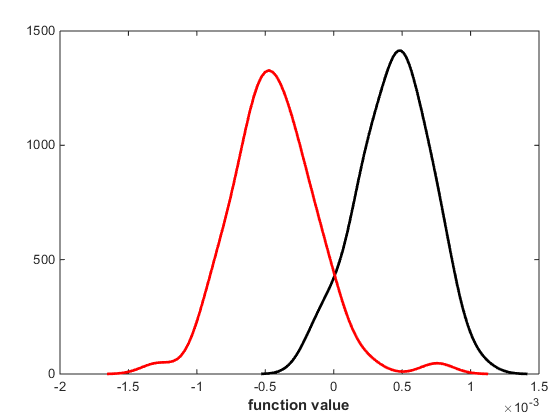
\includegraphics[width=8cm]{images/prt_ui_results_plots_hist.png}
\caption{Example function values histogram curve for a binary problem modelled by L1-MKL.}
\label{fig_prt_ui_results_plots_hist}
\end{center}
\end{figure}

\subsubsection{Confusion matrix plot}

The confusion matrix shows counts of predicted class labels $\hat{\omega}_n = f(\mathbf{x}_n)$ (in rows) versus true class labels $\omega_n$ (in columns). An ideal confusion matrix is diagonal: all predicted class labels correspond to the truth. Off-diagonal elements represent errors. It is important to check that none of the classes is
``sacrificed'' to gain accuracy in other classes - in other words, if all classes are equally
important to classify, no class should have more off-diagonal than on-diagonal entries. Many
summary statistics, including class accuracy, total accuracy, sensitivity, and specificity,
can be computed from the confusion matrix.

Figure \ref{fig_prt_ui_results_plots_confMat} shows an example of a confusion matrix (Haxby dataset, Faces versus Houses versus Scissors, LOBO CV).


\begin{figure}[h!]
\begin{center}
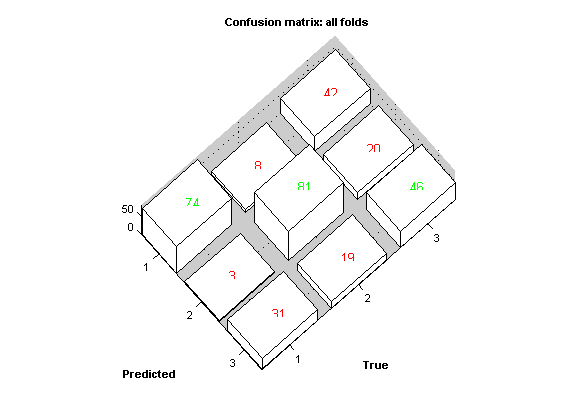
\includegraphics[height=6cm]{images/prt_ui_results_plots_confMat.png}
\caption{Example confusion matrix for all folds of a three-class problem modelled by GP.}
\label{fig_prt_ui_results_plots_confMat}
\end{center}
\end{figure}

\subsection{Regression}

\subsubsection{Predictions (scatter)}

This plot represents the predicted values (x-axis) against the real values or targets (y-axis). A perfect correspondence between targets and predictions would be represented by a diagonal on this plot. Figure \ref{fig_prt_ui_results_plots_predReg} displays such a plot for the prediction of age from sMRI images (IXI dataset, 15 images acquired across 3 centres).

\begin{figure}[h!]
\begin{center}
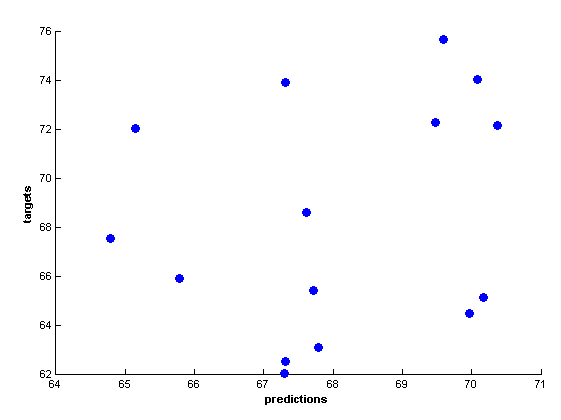
\includegraphics[height=6cm]{images/prt_ui_results_plots_predReg.png}
\caption{Example of scatter prediction plot on 15 data points modelled by KRR.}
\label{fig_prt_ui_results_plots_predReg}
\end{center}
\end{figure}

\subsubsection{Predictions (bar)}

This plot displays, for each image/subject, the target and the prediction in bar plots. An example plot is displayed in Figure \ref{fig_prt_ui_results_plots_bar} for the same model. 

\begin{figure}[h!]
\begin{center}
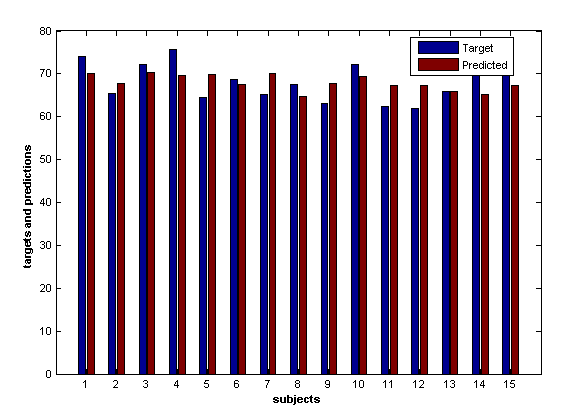
\includegraphics[height=6cm]{images/prt_ui_results_plots_bar.png}
\caption{Example of bar prediction plot on 15 data points modelled by KRR.}
\label{fig_prt_ui_results_plots_bar}
\end{center}
\end{figure}

\subsubsection{Predictions (line)}

This plot displays, for each fold, the target and the prediction, each in line plots. An example plot is displayed in Figure \ref{fig_prt_ui_results_plots_line} for the same model. 

\begin{figure}[h!]
\begin{center}
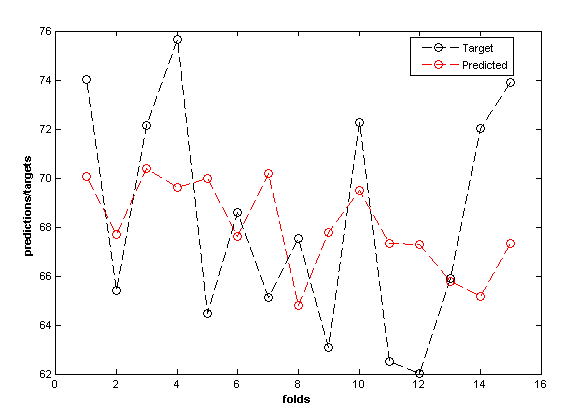
\includegraphics[height=6cm]{images/prt_ui_results_plots_line.png}
\caption{Example of line prediction plot on 15 data points modelled by KRR.}
\label{fig_prt_ui_results_plots_line}
\end{center}
\end{figure}

\subsection{Influence of the hyper-parameter on performance}

This plot will be present in the list if hyper-parameter optimization was performed. When displaying the average across folds, for each value of the hyper-parameter, it displays the average model performance (balanced accuracy for classification and MSE for regression, line on the plot) across nested folds, with an error bar representing the standard deviation of model performance. The frequency of selection of a hyper-parameter value (i.e. the number of times this value was returned as `optimal' to the outer CV fold) is represented with a gray bar plot on the right-side y-axis. An example of such a plot is displayed in Figure \ref{fig_prt_ui_results_plots_hyper} for the optimization of the soft-margin parameter in L1-MKL (Haxby dataset, Faces versus Houses, 4-folds nested CV, LOBO outer CV). When selecting a specific fold, this plot displays the model performance for each value of the hyper-parameter, and represents the optimal value (i.e. the one leading to highest performance) in red. 

\begin{figure}[h!]
\begin{center}
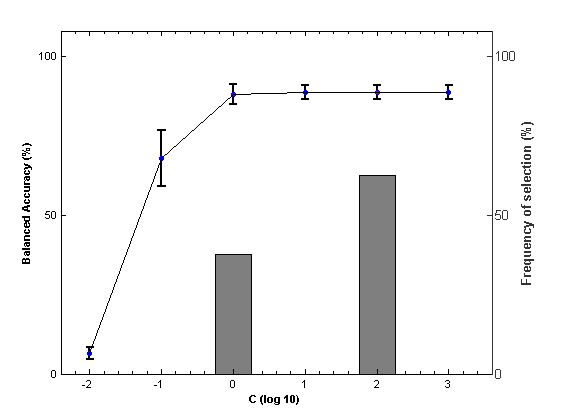
\includegraphics[height=6cm]{images/prt_ui_results_plots_hyper.png}
\caption{Example performance curve depending on the hyper-parameter value with frequency of selection of each hyper-parameter.}
\label{fig_prt_ui_results_plots_hyper}
\end{center}
\end{figure}

\section{Statistical analysis of a machine's performance}
\label{s:DisRes_stats}

One of the main questions to ask of a model is how precise its predictions are.
In regression, goodness-of-fit is often assessed via mean squared error and coefficient of determination ($R^2$). In classification, a common practice is to compute prediction accuracy, both for each class and for all test data. Once a specific performance metric has been obtained, it is also possible to obtain a p-value for the metric, reflecting
how certain we are that the result is not due to chance.

The statistics table gives a summary of the model's performance. Model performance is estimated differently for classification and for regression. In PRoNTo, classification performance is assessed using total accuracy (TA), balanced accuracy (BA), class accuracies (CA) and class predictive values. For regression, the goodness-of-fit is assessed based on the coefficient of determination ($R^2$), the mean squared error (MSE), the normalized mean squared error, and the correlation between the targets and the predictions.

\subsection{Classification} 

The accuracy $acc$ is the total number of correctly classified test samples divided by the total number of test samples $N$, irrespective of class. The accuracy is exactly equivalent to 

\begin{equation}
\label{eq:acc_as_01loss}
acc = 1- \frac{1}{N} \sum_n l_{01}(y_n,f(\mathbf{x}_n)),
\end{equation}

where $l_{01}(y_n,f(\mathbf{x}_n))$ is a 0-1 loss function that 
counts each classification error as costing 1 and each classification success as costing 0:

\begin{equation}
l_{01}(y_n,f(\mathbf{x}_n)) = \left\{
\begin{array}{ll}
0 & y_n = f(\mathbf{x}_n)\\
1 & y_n \neq f(\mathbf{x}_n)
\end{array} \right.
\end{equation}


Balanced accuracy takes the number of samples in each class into account, and gives equal weight
to the accuracies obtained on test samples of each class. In other words, the class-specific accuracy is computed by restricting 
the sum of equation \ref{eq:acc_as_01loss} to be taken over $C$ disjoint subsets of the whole testing data,
where each subset contains only test samples from one class. This produces a set of class-specific
accuracies $\{acc_1, \ldots, acc_C\}$, from which the balanced accuracy can be computed as 

\begin{equation}
acc^{bal}=\frac{1}{C} \sum acc_c .
\end{equation}

Balanced accuracy is the measure of choice when there is class imbalance (one
class, called the \textit{majority class}, has much more data than others).

The stats panel also gives the class accuracies $\{acc_1, \ldots, acc_C\}$, useful
to check whether the model favours some classes over others. If class 1 represents control subjects, 
and class 2 represents patients, then class 1 accuracy is equivalent to specificity, and class 2 accuracy is 
equivalent to sensitivity. In the same way, the figure displays class positive predictive value, which represents the number of false positives for each class. An example of classification stats is displayed in Figure \ref{fig_prt_ui_results_statsTable}.

\begin{figure}[h!]
\begin{center}
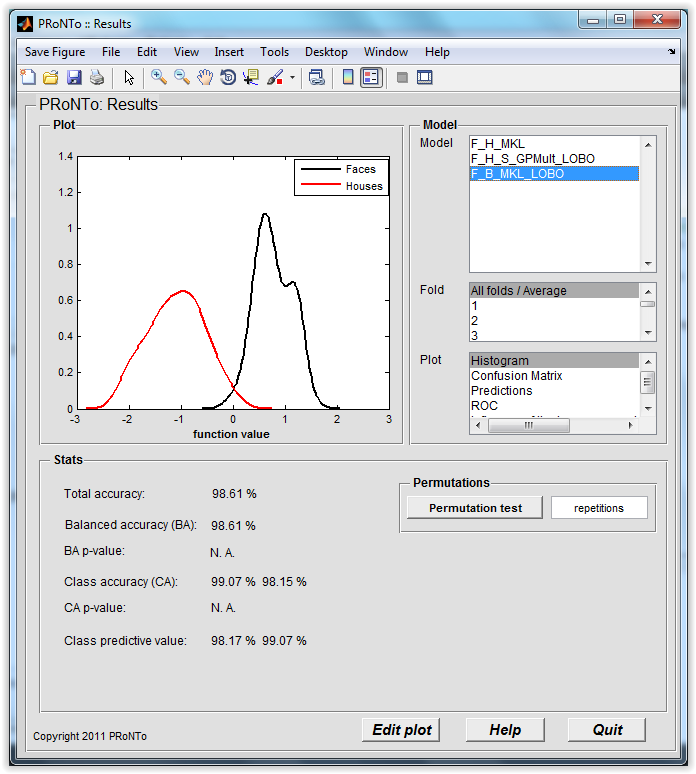
\includegraphics[height=8cm]{images/prt_ui_results_statsTable.png}
\caption{Example statistics for all folds of a two-class problem modelled by an L1-MKL.}
\label{fig_prt_ui_results_statsTable}
\end{center}
\end{figure}

\subsection{Regression}

As previously mentioned, model performance for regression is assessed by the correlation between the predictions and the targets (linear correlation), the coefficient of determination ($R^2$), the mean square error (MSE), and the normalized MSE. An example of such stats window is displayed in Figure \ref{fig_prt_ui_results_statsTableReg}.

\begin{figure}[h!]
\begin{center}
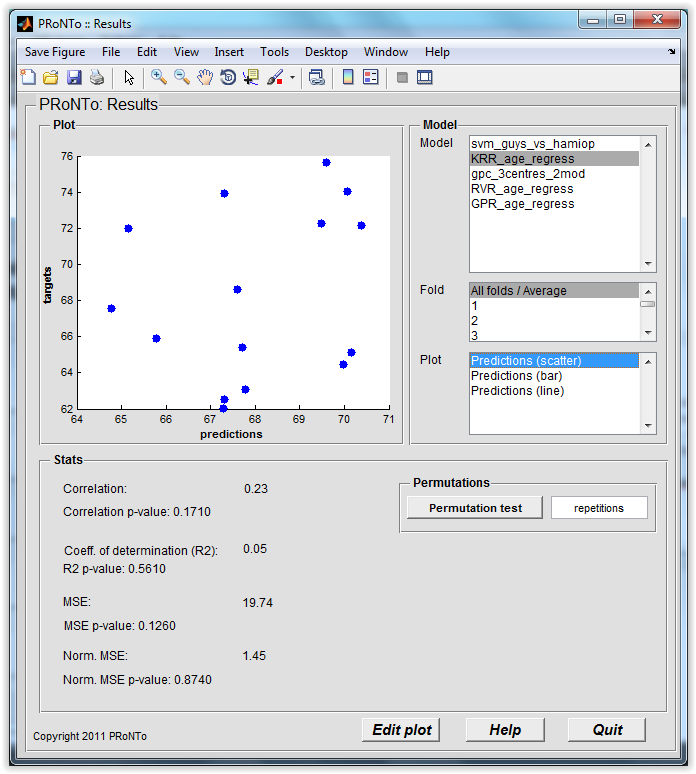
\includegraphics[height=8cm]{images/prt_ui_results_statsTableReg.PNG}
\caption{Example statistics for all folds of a KRR modelling on 15 data points.}
\label{fig_prt_ui_results_statsTableReg}
\end{center}
\end{figure}

% We have the following fields in stats, stats.r2 'Coefficient of Determination', stats.mse 'Mean Squared Error', stats.nmse 'Normalised Mean Squared Error', all calculated in prt_stats.m
The mean-squared error is calculated as:
\begin{equation}
\begin{aligned}
MSE=\frac{1}{N}\sum_{n} (y_n-f(\mathbf{x}_n))^2
\end{aligned}
\end{equation}
This is the standard measure when assessing goodness-of-fit for regression models. 
%There are two important things to remember when using this measure. Firstly, its value is disproportionately affected by bad predictions, because of the 'squared' term. Secondly, its value will be affected by the range of y ie. ....
%Note that the value of this measure is affected by the scale of y. 
%We therefore also calculate 
%the Normalised Mean Square Error, `NMSE':
Since the magnitude of the MSE depends on the scale of $y$, we also calculate the Normalised Mean Square Error, `Norm. MSE':
\begin{equation}
\begin{aligned}
Norm. MSE=\frac{MSE}{(y_{max}-y_{min})}
\end{aligned}
\end{equation}
where we divide the MSE by the range of the targets over the 
%ie., training and test, 
data. This gives a scale invariant measure of prediction accuracy.
In addition, the correlation coefficient of the targets and predictions are determined:
\begin{equation}
\begin{aligned}
CORR=\frac{\sum_{n} (y_n-\mu_y) (f(\boldsymbol{x}_n)-\mu_f)}{\left\{\sum_{n} (y_n-\mu_y)^2 \sum_{n} (f(\boldsymbol{x}_n)-\mu_f)^2\right\}^\frac{1}{2}}
\end{aligned}
\end{equation}
in which $\mu_y$ and $\mu_f$ are the sample means of the targets and predictions respectively. The resulting measure $-1<CORR<1$ provides a measure of the strength of the linear dependence between the targets and the predicted targets, with values close to zero indicating no relationship, values close to 1 indicating a positive relationship, and values close to -1 indicating a negative relationship. Values of $CORR$ less than zero would imply that the model has performed poorly, as this would mean that targets with large values tend to be given smaller predicted values than targets with small values. However, it should be remembered that a large positive value of $CORR$ does not \emph{necessarily} mean that the model is giving accurate predictions, since 
%multiplying all the predictions by a constant scaling factor gives the same value for $CORR$. 
a global scaling and shifting of the predictions gives the same value for $CORR$. 
We would therefore recommend examining both $CORR$ and $MSE$, as well as the scatterplots, to verify that the model is performing well.  For completeness, the statistics table also include the `coefficient of determination' $R^2$, which is given by
\begin{equation}
\begin{aligned}
R^2=CORR^2
\end{aligned}
\end{equation}


\subsection{Permutation testing}

Much of statistical theory and machine learning theory rests on the assumption that the data is
IID (independently and identically distributed). However, in functional neuroimaging this assumption
is often not met, due to e.g. within-run correlations and haemodynamic effects. Therefore, classical estimates of
confidence intervals (such as the binomial confidence interval) may not always
be appropriate. Permutation testing is a non-parametric procedure that allows to obtain meaningful 
confidence intervals and p-values in this case. Because it requires retraining the model a number of times, 
which can be costly in computation time, this is not done by default. After filling in the {\tt repetitions}
field with a number of repetitions $R$, pressing the {\tt Permutation test} button will estimate the model for the specified number of times with permuted labels/targets, and produce a  p-value for performance statistics (see Figure~\ref{fig_prt_ui_results_statsTable}). The smallest increment in p-value is equal to $1/R$ (e.g. 20 permutations gives you increments of 0.05), with a minimum value of $1/R$ (i.e. running 10 permutations will never lead to statistically significant result at the commonly used threshold of $p<0.05$). Usually, we would recommend computing several hundreds to a thousand permutations.

For both classification and regression models, the p-value associated with each performance measure can be estimated using permutations. Until they have been estimated, `N.A.' will be displayed (standing for `not available').

\textbf{Important note:} This step is essential to assess model performance! It is not methodologically sound to simply assume that the chance level is close to $50\%$ and that any balanced accuracy higher than that threshold is significant. Please report p-values as computed from permutations along with model performance.

% XXX Maybe ref Golland TR

